\begin{frame}
    \centering
    \begin{figure}[H]
        
\includegraphics[keepaspectratio, width=0.7\paperwidth, height=\paperheight]{LeeLogo}
    \end{figure}
    Informatik: Programmieren\\
    \emoji{turtle} Kapitel 01: \textbf{Einführung}
\end{frame}

\begin{frame}{Einführung}
Was erwartet Sie?
\begin{itemize}
\item \textbf{Programmieren}: Grundkonzepte (Schleifen, Verzweigungen, Variablen)
\item \textbf{Robotik}: Steuerung von Technik (Roboter, Sensoren, Aktoren)
\end{itemize}
\end{frame}



\begin{frame}[fragile]{Lehrmittel}
\begin{columns}
\begin{column}{.2\pagewidth}
\begin{figure}[H]
\centering

\includegraphics[width=.8\columnwidth]{GrundlagenInfo/00_Programmieren/Figures/Book}
\end{figure}
\end{column}

\begin{column}{.6\pagewidth}
Arten von Aufgaben im Buch
\begin{itemize}
\item 
\includegraphics[width=0.1\linewidth]{GrundlagenInfo/00_Programmieren/Figures/book-tasks-1} ``Normale Aufgaben'' $\rightarrow$ prüfungsrelevant
\item 
\includegraphics[width=0.1\linewidth]{GrundlagenInfo/00_Programmieren/Figures/book-tasks-2} ``Challenge-Aufgaben''
\item 
\includegraphics[width=0.1\linewidth]{GrundlagenInfo/00_Programmieren/Figures/book-tasks-3} Vertiefung \& Prüfungsvorbereitung
\end{itemize}
\end{column}
\end{columns}
\vspace{.5cm}

\begin{itemize}
\item Kosten: 23.20
\item Lösungen und Zusatzmaterialien auf \href{https://www.klett.ch/login/schueler/registrieren}{meinklett.ch}
\item Registrierung mit Schlüssel im Buchumschlag
\end{itemize}
\end{frame}

\begin{frame}{Was ist Programmieren?}
\begin{itemize}[<+->]
\item \emoji{light-bulb} Seine Gedanken logisch ausdrücken
\begin{displayquote}
``The truth is you don’t really understand something until you’ve taught it to a computer, until you’ve been able to program it.'' --- Donald Knuth, PhD
\end{displayquote}
\item \emoji{otter} Dem Computer Befehle / Aufträge geben

\item \emoji{desert-island} Automatisieren \& das Leben vereinfachen

\end{itemize}
\end{frame}

\begin{frame}{Programmieren: Demo}
\end{frame}

\begin{frame}[fragile]{Programmieren: Erste \textbf{Befehle}}
\begin{table}[H]
\centering
\footnotesize
\begin{tabular}{l|l|p{4cm}}
\textbf{Befehl} & \textbf{Abkürzung} & \textbf{Bedeutung} \\\midrule\midrule
\lstinline[style=TigerJython]|from gturtle import *| &  & Alle nötigen Funktionen ``laden‘‘ \\\midrule
\lstinline[style=TigerJython]|makeTurtle()| &  & Turtle erstellen \\\midrule
\lstinline[style=TigerJython]|hideTurtle()| &  & Turtle verstecken, Resultat direkt zeigen \\\midrule
\lstinline[style=TigerJython]|forward(100)| & \lstinline[style=TigerJython]|fd(100)| & Gehe 100 Pixel nach vorne   \\\midrule
\lstinline[style=TigerJython]|left(90)| & \lstinline[style=TigerJython]|lt(90)| & Um 90 Grad nach links drehen   \\\midrule
\lstinline[style=TigerJython]|right(90)| & \lstinline[style=TigerJython]|rt(90)| & Um 90 Grad nach rechts drehen   \\\midrule
\lstinline[style=TigerJython]|setPenColor("green")| & \lstinline[style=TigerJython]|spc("green")| & Stiftfarbe auf grün setzen  \\\midrule
\lstinline[style=TigerJython]|setPenWidth(2)| & \lstinline[style=TigerJython]|spw(2)| & Stift-Dicke auf 2 setzen  \\
\end{tabular}
\end{table}

\textbf{Allgemein}: \lstinline[style=TigerJython]|befehlsname(p1, p2, ...)|
\end{frame}


\begin{frame}[fragile]{Programmieren: Erste \textbf{Schleifen}}
\begin{lstlisting}[style=TigerJython,escapechar=!]
from gturtle import *
makeTurtle()

repeat 6:     !\tikzmark{repeatStart}!
    fd(100)   !\tikzmark{bodyStart}!
    rt(360/6) !\tikzmark{bodyEnd}!
\end{lstlisting}
\begin{tikzpicture}[overlay, remember picture,
    every edge/.append style = { ->, thick, >=stealth, red!70},
    every node/.style={draw=red!50,fill=red!50!white,text=black,rounded corners}]
    \only<2->{\drawBrace{1em}{repeatStart}{bodyEnd}{Schleife}{.3}{};}
    \only<3->{\drawBrace{.0em}{bodyStart}{bodyEnd}{\textit{Körper} der Schleife}{.7}{};}
\end{tikzpicture}

\end{frame}



\begin{frame}{Zusammenfassung}
\begin{itemize}[<+->]
\item Mit \textbf{Befehlen} können wir den Computer eine abstrakte Tätigkeit ausführen lassen
\item \textbf{Parameter} dienen dazu, die Befehle \textit{parametrisieren} (Analogie: Kochrezept für 2 oder 4 Personen)
\item \textbf{Schleifen} erlauben es, repetitive Tätigkeiten kompakt zu beschreiben
\item Unterschiedliche \textbf{Datentypen} für unterschiedliche Zwecke
\end{itemize}
\end{frame}

\begin{frame}[fragile]{Auftrag}
\begin{itemize}
\item \aufgabebox{Buch, Aufgaben 1.1 bis 1.14 (S. 6-13)}
\item \abgabebox{Buch, Aufgaben 1.7 und 1.13: Abgabe auf Moodle}
\item \challengebox{Moodle, Challenge-Aufgabe ``Schachbrett''}
\end{itemize}
\end{frame}

\begin{frame}[fragile]{Schleifen in Schleifen}{Demo: Blume}

\begin{lstlisting}[style=TigerJython,escapechar=!]
from gturtle import *
makeTurtle()
hideTurtle()

repeat 10:
    # mach ein Viereck
    repeat 4:
        fd(100)
        rt(360/4)

    # leichte Rechtsdrehung
    rt(360/10)
\end{lstlisting}
\begin{figure}[H]
\centering
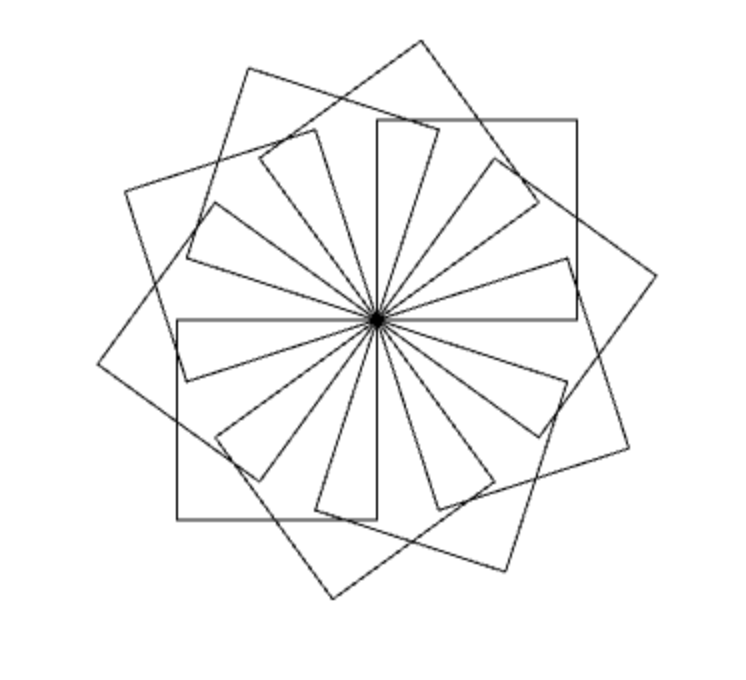
\includegraphics[width=0.2\pagewidth]{GrundlagenInfo/00_Programmieren/Figures/viereck_blume}
\end{figure}
\end{frame}

\begin{frame}[fragile]{Schleifen in Schleifen}{Weitere Beispiele aus dem Buch}
\begin{itemize}
\item Beispiel 1.8
\item Beispiel 1.9
\end{itemize}
\end{frame}

\begin{frame}[fragile]{Auftrag}
\begin{itemize}
\item \aufgabebox{Buch, Aufgaben 1.15 bis 1.19}
\item \abgabebox{Aufgabe 1.18: Abgabe auf Moodle}
\end{itemize}
\end{frame}

\begin{frame}[fragile]{Datentypen}
\begin{table}[H]
\footnotesize
\centering
\begin{tabular}{l|p{2cm}|p{2cm}}
\textbf{Beispiel} & \textbf{Datentyp (englisch, Abk.)} & \textbf{Datentyp (Deutsch)} \\\midrule\midrule
\lstinline[style=TigerJython]|"Hallo Welt", "abc", "42"| & string (str) & Zeichenkette \\\midrule
\lstinline[style=TigerJython]|15, 45, -5, 0| & integer (int) & Ganzzahl \\\midrule
\lstinline[style=TigerJython]|12.23, -5.33, 23.0| & float (float) & Kommazahl
\end{tabular}
\end{table}

\textbf{Analogie}:
\begin{itemize}
\item Name (string)
\item Alter in Jahren (integer)
\item Grösse in Metern (float)
\end{itemize}
\end{frame}

\begin{frame}[fragile]{Auftrag}
\begin{itemize}
\item \aufgabebox{Buch, Aufgaben 1.20 bis 1.28}
\item \abgabebox{Aufgabe 1.20: Abgabe auf Moodle}
\item Tipp: Backslash (\textbackslash) 
\begin{itemize}
\item auf MacOS: \keys{\shift+\Alt+7}
\item auf Windows: \keys{\AltGr+\textbackslash}
\end{itemize}
\end{itemize}
\end{frame}